\section{Two-Period Labor Supply}


A consumer lives for two periods with preferences
\begin{equation}
  V = \sum_{t=1}^2 \beta^{t-1} \left( \frac{c_t^{1-\sigma}}{1-\sigma} - \frac{h_t^{1+\gamma}}{1+\gamma} \right),
\end{equation}
where $\sigma$ is the inverse elasticity of intertemporal substitution and $\gamma$ is the inverse Frisch elasticity of labor supply. The consumer saves in a riskless asset with interest rate $r$ and receives income $T + (1-\tau) W e_t h_t$ in period $t$. The budget constraints are
\begin{align}
  c_1 + a_2 &= T + (1-\tau) W e_1 h_1, \\
  c_2 &= T + (1-\tau) W e_2 h_2 + (1+r) a_2.
\end{align}
Efficiency is normalized to $e_1 = 1$ in the first period and equals $e_2$ in the second; we solve for different values of $e_2$. The consumer cannot borrow:
\begin{equation}
  a_2 \ge 0.
\end{equation}

\paragraph{Parameters.}
We use $\beta = 0.90$, $\sigma = 1.5$, $\gamma = 2$, $r = 0.04$, $W = 1$, $\tau = 0.25$, $T = 0.15$.

\subsection{Backward induction and optimality conditions}

The problem is solved by backward induction, respecting the no-borrowing constraint. In period 2, the consumer enters with assets $a$ and chooses $(c_2, h_2)$ subject to the budget constraint and the labor-leisure first-order condition. In period 1, the consumer chooses $(c_1, h_1)$ (and hence $a_2$) to maximize lifetime utility, subject to $a_2 \ge 0$.

\paragraph{Period 2.}
The labor-leisure FOC is
\begin{equation}
  h_2^\gamma = (1-\tau) W e_2\, c_2^{-\sigma}.
\end{equation}
With $c_2 = T + (1-\tau) W e_2 h_2 + (1+r) a$, substituting the budget into the FOC yields a single equation in $c_2$. Equivalently, define next-period assets as a function of current consumption and (implied) hours:
\begin{equation}
  a' = T + (1-\tau) W e h + (1+r) a - c.
\end{equation}
Given $c$, hours are backed out from the FOC: $h = \bigl( (1-\tau) W e\, c^{-\sigma} \bigr)^{1/\gamma}$. At the end of life we require $a_3 = 0$, so we solve for $c_2$ such that $a'(c_2) = 0$. This yields $c_2(a,e_2)$, $h_2(a,e_2)$, and the period-2 value
\begin{equation}
  V_2(a,e_2) = \frac{c_2(a,e_2)^{1-\sigma}}{1-\sigma} - \frac{h_2(a,e_2)^{1+\gamma}}{1+\gamma}.
\end{equation}

\paragraph{Period 1.}
For any $c_1$, hours satisfy $h_1^\gamma = (1-\tau) W e_1 c_1^{-\sigma}$ (with $e_1=1$) and savings are
\begin{equation}
  a_2 = T + (1-\tau) W e_1 h_1 - c_1.
\end{equation}
The upper bound $\bar{c}_1$ such that $a_2(\bar{c}_1) = 0$ ensures the no-borrowing constraint when we restrict $c_1 \in (0, \bar{c}_1]$. The consumer solves
\begin{equation}
  \max_{c_1 \in (0,\bar{c}_1]} \quad \frac{c_1^{1-\sigma}}{1-\sigma} - \frac{h_1^{1+\gamma}}{1+\gamma} + \beta V_2(a_2, e_2).
\end{equation}
At an interior optimum the Euler equation holds: $c_1^{-\sigma} = \beta(1+r) c_2^{-\sigma}$.

\subsection{Numerical solution: period 2}

We implement the period-2 solution as follows. For each pair $(a, e_2)$ on a grid, we find $c_2$ such that $a'(c_2) = 0$ using a bisection root-finder on the function \texttt{savings}$(c, a, e_2, p)$, which returns $a'$ given consumption (and implied hours from the labor FOC). This yields $c_2(a,e_2)$, $h_2(a,e_2)$, and $V_2(a,e_2)$.

\begin{algorithm}[H]
\caption{Period-2 solution (for each $(a,e_2)$)}
\label{alg:problem4-period2}
\begin{algorithmic}[1]
\State \textbf{Input:} Asset grid $a$, productivity $e_2$, parameters $p$
\State \textbf{Output:} $c_2(a,e_2)$, $h_2(a,e_2)$, $V_2(a,e_2)$
\For{each $(a_i, e_2)$}
  \State Bracket $c \in (0, \overline{\text{coh}})$ so that \texttt{savings}$(c,a_i,e_2,p)$ has a root
  \State $c_2 \gets \texttt{bisect}(\texttt{savings}, \ell, u; a_i, e_2, p)$ so that $a' = 0$
  \State $h_2 \gets$ hours from labor FOC given $c_2$
  \State $V_2 \gets u(c_2,h_2)$
\EndFor
\State \textbf{return} $V_2$, $c_2$, $h_2$
\end{algorithmic}
\end{algorithm}

\Cref{fig:problem4-period2} shows the period-2 consumption, hours, and value as surfaces over $(a, e_2)$.

\begin{figure}[H]
\centering
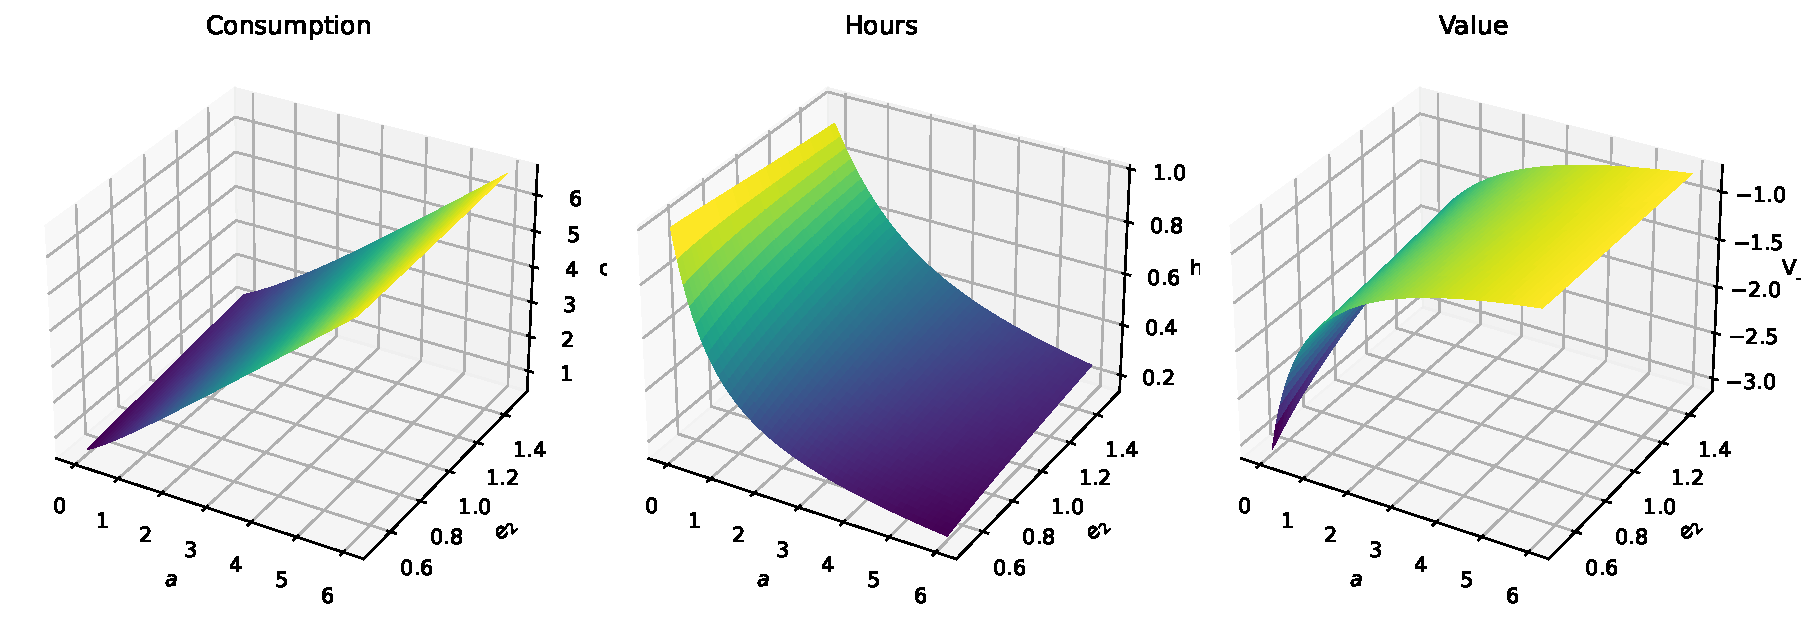
\includegraphics[width=\textwidth]{figures/problem4_period2_surfaces}
\caption{Period-2 policy and value: $c_2(a,e_2)$, $h_2(a,e_2)$, and $V_2(a,e_2)$ on a grid of assets $a$ and second-period productivity $e_2$.}
\label{fig:problem4-period2}
\end{figure}

\subsection{Numerical solution: period 1}

Given the period-2 value and policies, we solve the period-1 problem for each $e_2$ in a grid. Step (A): find the maximum feasible period-1 consumption $\bar{c}_1$ such that $a_2 = 0$ (bisection on \texttt{savings}$(c, 0, 1, p)$ with $a_1=0$, $e_1=1$). Step (B): maximize the period-1 lifetime value over $c_1 \in (0, \bar{c}_1]$ using golden-section search on the function that returns $u(c_1,h_1) + \beta V_2(a_2, e_2)$. Step (C): from the optimal $c_1$ we recover $h_1$, $a_2$, and then $c_2$, $h_2$ from the period-2 solution at $(a_2, e_2)$.

\begin{algorithm}[H]
\caption{Period-1 solution (for each $e_2$)}
\label{alg:problem4-period1}
\begin{algorithmic}[1]
\State \textbf{Input:} Productivity grid $e_2$, parameters $p$
\State \textbf{Output:} $c_1(e_2)$, $h_1(e_2)$, $a_2(e_2)$, $c_2(e_2)$, $h_2(e_2)$
\For{each $e_2$}
  \State $\bar{c}_1 \gets \texttt{bisect}(\texttt{savings}, \ell, u; 0, 1, p)$ so that $a_2 = 0$
  \State $c_1^* \gets \argmax_{c_1 \in (0,\bar{c}_1]} \bigl\{ u(c_1,h_1) + \beta V_2(a_2,e_2) \bigr\}$ via \texttt{golden\_search} on minus the objective
  \State $h_1 \gets$ hours from labor FOC; $a_2 \gets$ \texttt{savings}$(c_1^*, 0, 1, p)$
  \State $(c_2, h_2) \gets$ period-2 solution at $(a_2, e_2)$
\EndFor
\State \textbf{return} $c_1$, $h_1$, $a_2$, $c_2$, $h_2$
\end{algorithmic}
\end{algorithm}

The policy functions we report are expressed as functions of $e_2$ only. This is because we condition on the asset choice $a_2$ being the one chosen optimally in period 1 given $e_2$ (and $a_1=0$). So for each $e_2$, the plotted $c_1$, $h_1$, $a_2$, $c_2$, $h_2$ are the equilibrium choices along that path; they are not the full policy functions $c_2(a,e_2)$ and $h_2(a,e_2)$ over all $a$, but the realized consumption and hours given the endogenous $a_2(e_2)$.

We plot consumption, hours, and assets only for \emph{interior} points where $a_2 > 0$ (non-binding borrowing constraint), so that the Euler equation is approximately satisfied and the curves are smooth.

\begin{figure}[H]
\centering
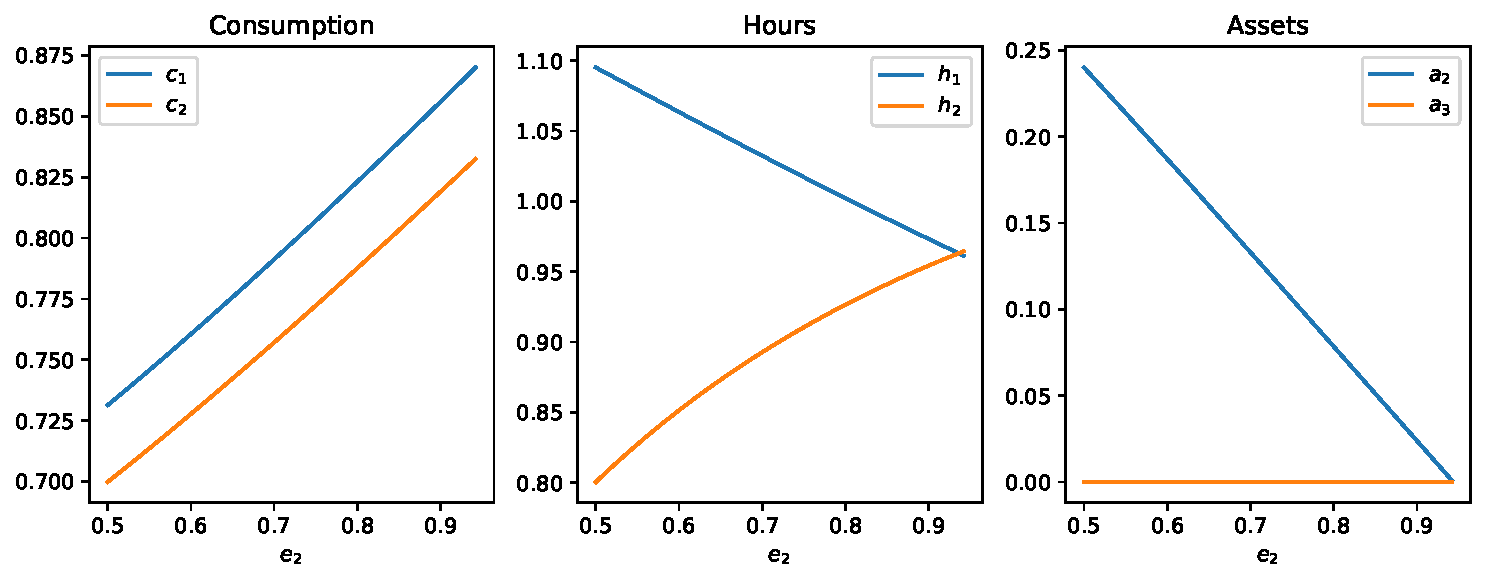
\includegraphics[width=\textwidth]{figures/problem4_policy_functions}
\caption{Period-1 policy functions as functions of $e_2$: consumption ($c_1$, $c_2$), hours ($h_1$, $h_2$), and assets ($a_2$, $a_3$). Plotted only where $a_2 > 0$ (interior). The second-period choices are evaluated at the endogenously chosen $a_2(e_2)$.}
\label{fig:problem4-policy}
\end{figure}
